%# -*- coding: utf-8-unix -*-
%%==================================================
%% chapter02.tex for SJTU Master Thesis
%% Encoding: UTF-8
%%==================================================

%1,展开差分隐私定义,laplace,讨论维度问题
%2,展开面向决策树的差分隐私设计,典型方案


\chapter{相关背景技术}
\label{chap:background}

\section{引言}

上一章描述了课题所涉及的背景知识及相关问题的研究现状,本章将介绍差分隐私理论知识及焦点问题。主要内容为差分隐私相关的数学定义、重要概念介绍和问题本质模型的描述。

\section{差分隐私}

\subsection{差分隐私定义}

%给定数据集$D$,另一数据集$D'$和它至多相差一条记录。
在差分隐私中,我们希望某个在数据集上的运算结果不因任意一条记录的改变而变化明显。也就是说,某个算法在改变前后的两个数据集上做运算,其输出上的差别不至于披露任意一条特定数据项。

\begin{defn}
	
($\varepsilon$\textsc{-差分隐私})\supercite{Dwork Calibrating} 数据集$D$和$D'$至多相差一条记录,即$|D$$\triangle$$D'|$ $\leqslant$ 1。一个随机算法$\partial$满足$\varepsilon$-差分隐私,当且仅当对于$\partial$任意可能的输出$O$,我们有下式成立:

\begin{equation}
  \label{eq:res1}
	 Pr[\partial(D) = O] \leqslant e^{\varepsilon} \cdot Pr[\partial(D') = O]
\end{equation}


其中,$Pr$表示事件发生的概率,在此也表示隐私被披露的风险。$\varepsilon$为隐私预算,$\varepsilon$越小,算法的隐私保护程度越高。

\end{defn}

实现差分隐私的主要方法是对真实值添加噪音扰动,而噪音量的量级大小是由全局敏感性(Sensitivity)来定义。它表示数据集发生改变时,某一函数运算在输出结果上产生的最大距离。

\begin{defn}
	(\textsc{全局敏感性}\supercite{Dwork Calibrating}) 数据集$D$和$D'$至多相差一条记录,即$|D$$\triangle$$D'|$ $\leqslant$ 1。函数$\mathcal{F}$的查询维度为d,并且有$\mathcal{F}$:$D \rightarrow \mathrm{R}^d$。那么,函数$\mathcal{F}$的全局敏感性$S(\mathcal{F})$定义为:
\begin{equation}
\label{eq:res2}
	S(\mathcal{F}) = \max \limits_{D,D'} \| \mathcal{F}(D) - \mathcal{F}(D') \|_{1}
\end{equation}

其中,$\|\cdot\|$表示$L_{1}$范数。
\end{defn}

\subsection{差分隐私实现机制}

基于全局敏感性,本课题涉及两种加噪算法:拉普拉斯机制(Laplace mechanism)和指数机制(Exponential mechanism)。

\begin{thm}
	\label{thm:res1}
	(\textsc{拉普拉斯机制}\supercite{Dwork Calibrating}) 在数据集$D$中,有函数$\mathcal{F}$: $D\rightarrow \mathrm{R}^d$,若算法$\mathcal{M}$满足下式,则$\mathcal{M}$满足$\varepsilon$-差分隐私:
	\begin{equation}
	\mathcal{M}(D) = \mathcal{F}(D) + (\textit{Laplace}(S(\mathcal{F})/ \varepsilon)^d
	\end{equation}
	其中,\textit{Laplace}为标准的拉普拉斯分布,$S(\mathcal{F})/\varepsilon$决定噪音量级。
\end{thm}
例如,当$\mathcal{F}$为求和函数时,S($\mathcal{F}$)=1,此时$\mathcal{M}(D) = \mathcal{F}(D) + (\textit{Laplace}(1/\varepsilon)^d$。

指数机制通过设计打分函数对属性进行打分计算,分值越高就有越大的概率被选中。
\begin{thm}
	\label{thm:res2}
	(\textsc{指数机制}\supercite{exponential}) 有数据集$D$,打分函数$\mathcal{F}$: ($D$ $\times$ $O$)$\rightarrow$ $\mathrm{R}$,对每个输出项o$\in$ $O$都对应一个打分值。对于若算法$\mathcal{M}$满足下式,则$\mathcal{M}$满足$\varepsilon$-差分隐私:
	\begin{equation}
	\mathcal{M}(D,\mathcal{F}) = \{o \in O: Pr(o)\wasypropto exp(\frac{\varepsilon\mathcal{F}(D,o)}{2S(\mathcal{F})}) \}
	\end{equation}
	其中,S($\mathcal{F}$)为打分函数$\mathcal{F}$的全局敏感性,Pr(o)表示返回输出项o的概率。
\end{thm}
在决策树分类算法中,常用的打分有信息增益,基尼指数等。通过算法$\mathcal{M}$得到候选属性的概率值分布,之后按照概率抽取属性。

\subsection{差分隐私性质与准确度损失}

\subsubsection{差分隐私性质}
对于不同组合关系的数据集,差分隐私具有序列(垂直)组合性质和并行(水平)组合性质。

\begin{lem}
	序列组合性质(Sequential composition)\supercite{composition}随机算法$A_{i}$满足$\varepsilon_{i}$-差分隐私,则一系列算法$A_{i}$在数据集$D$上的序列组合满足$\sum\limits_i \varepsilon_{i}$-差分隐私。
\end{lem}

\begin{lem}
	\label{parallel}
	并行组合性质(Parallel composition)\supercite{composition}随机算法$A$满足$\varepsilon$-差分隐私,数据集$D$被划分为一系列不相交的子集$D_{i}$,则算法$A$在每个数据集$D_{i}$上的操作$A(D_{i})$均满足$\varepsilon$-差分隐私。
\end{lem}

\subsubsection{误差方差}
噪音的引入虽然满足了差分隐私定义,但降低了数据集的准确性,那么如何量化这一准确度损失呢?误差方差是常用的度量稳定性的计算指标,以原数据集分布为准,与加噪结果分布间的误差方差也就是真实值的偏离程度。因此,在本课题研究中使用误差方差作为量化发布数据(加噪数据)准确度损失的指标,衡量其可用性。
定义如下。
\begin{defn}
	\label{thm:error}
	(\textsc{误差方差}$error_{var}$\supercite{Dwork Calibrating}) 在数据集$D$中,有查询函数$\mathcal{F}$: $D\rightarrow \mathrm{R}^d$且满足拉普拉斯机制,$\mathbb{E}$为方差,则查询的第i个元素的误差方差$error_{var}^{i}$及对整个查询Q的误差方差为
	\begin{eqnarray}
	&error_{var}^{i} = \mathbb{E}(\textit{Laplace}(S(\mathcal{F})/ \varepsilon)^2) = 2\frac{S(\mathcal{F})^2}{\varepsilon^2}\\
	&error_{var}^{Q} = \sum\nolimits_{i \in Q}error_{var}^{i}
	\end{eqnarray}
	其中,\textit{Laplace}为标准的拉普拉斯分布,$S(\mathcal{F})$为全局敏感性。
\end{defn}

例如,当$\mathcal{F}$为计数函数时全局敏感性为1,对于n个元素的查询Q,$error_{var}^{Q}$ = n$\mathbb{E}(\textit{Laplace}(S(1)/ \varepsilon)^2)$ = 2n/$\varepsilon^2$。

\section{频率矩阵及问题表述}

频率矩阵是数据处理中一种基本的统计模型,在面向分类应用的处理中被广泛使用到。基于频率矩阵实现的差分隐私算法满足了隐私保护需求,但分类应用中的范围计数查询需求引发了新问题---基于单位行项的应答查询模式引起了噪音线性叠加问题。%随着查询维度的增加,累加的噪音值不断逼近真实值,严重影响数据使用性能的扩展性---这也是本课题的焦点问题。
本节先介绍频率矩阵模型,接着对数据维度、查询维度进行量化表述,并分析频率矩阵的应答查询模式。

\subsection{频率矩阵}

继续以例\ref{exmp_cuboid}为示例,原表的频率矩阵即为取全属性时的立方表Cuboid{性别,年龄,成绩}。如图\ref{fig2:frequency}(a)为原表,\ref{fig2:frequency}(b)为其对应的频率矩阵。可以看到,频率矩阵是枚举原表中所有属性(包括类属性)的组合情况,并统计相关的计数情况,通常情况下频率矩阵是大于原表的。

\begin{figure}[!htp]
	\centering
	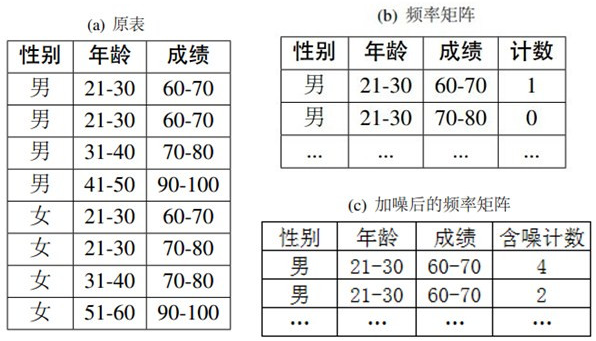
\includegraphics[width=5in]{chap2/frequency}
	\bicaption[fig2:frequency]{图}{频率矩阵示例}{Fig.}{Sample frequency matrix}
\end{figure}

频率矩阵对原表条目进行了组织,便于数据的管理和查询。因此,本文的“数据集”通指组织成频率矩阵形式的数据集,而不是原表。频率矩阵中的每一行称之为“行项”(entry),如表\ref{fig2:frequency}(b)的\{“男”,21-30,60-70,1\}为一个行项。

\subsection{频率矩阵加噪模型}

本章节将对\ref{sec:weidu}节的查询维度问题进行量化表述,并说明基于频率矩阵的差分隐私算法的应答查询模式。

\subsubsection{数据维度}
数据维度在差分隐私算法研究中一般用数据域尺寸(Domain size)来表示。数据集D有n个非空行项,n$\in$ Z$^{+}$,并且有d个属性\{A$_{1}$,A$_{2}$,...,A$_{d}$\},每个属性A$_{i}$(i=1,2,...,d)有|A$_{i}$|个属性值。D的数据域尺寸表示为M,则M = \(\prod\limits_{i = 1}^d {|A{_i} |}\)且M $\gg$ n。

\subsubsection{查询维度}
查询维度是由查询项所涉及的属性数目决定。查询请求Q(A$_{k}$, A$_{k+1}$, ..., A$_{j}$),其中j,k$\in$ Z$^{+}$,j $\geqslant$ k且j $\geqslant$ d,则Q的查询维度为$j-k$。

\subsubsection{应答查询模式}
\label{chap2_Linaer}

应答查询模式在本课题研究中指的是,为响应分类应用的范围计数查询需求所采用的查表、累加等操作并最终返回应答结果的方式。频率矩阵的应答查询模式由其数据组织方式决定,它查找符合查询范围的相关行项并对每个行项的计数值做累加运算,最后返回运算结果。以下定义频率矩阵的应答查询模式$LinearR$。

\begin{defn}
	(\textsc{线性累加的应答查询模式$LinearR$}) 有d维类属性分布的数据集$D$,范围查询$R_{query}$,对于其中某数据项$D_{i}$,查询函数$\mathcal{F}$:$D_{i} \rightarrow \mathrm{R}^d$,应答返回集合$Answer$,线性累加的应答查询模式$LinearR$定义为:
	\begin{equation*}
	\label{eq:linear_response}
		\begin{split}
			\text{当}\forall D_{i},D_{j} \in Answer, i \neq j, \text{则} D_{i} &\cap D_{j} = \varnothing,\text{且 }
			R_{query} = \bigcup\limits_{\forall D_{i} \in Answer} D_{i}\\
			\text{那么,有}LinearR &= \sum\limits_{\forall D_{i} \in Answer} \mathcal{F}(D_{i})
		\end{split}
	\end{equation*}
\end{defn}

在$LinearR$中,由于单个行项之间是互不相交的(在每个属性上具有不同的属性值分布),因此这种应答结果是以行项为单位的累加计算之和。

\subsubsection{频率矩阵加噪模型}

频率矩阵加噪模型是本课题所要改进的算法的问题模型,在下个章节会通过详例说明二者联系。

某查询请求Q'是对\{A$_{k}$, A$_{k+1}$, ..., A$_{j}$\}(Q)以外的某一属性值的查询,那么根据频率矩阵特性,在D中查表涉及到的行项数至少为E = \(\prod\nolimits_{i \in (1,d) - (k,j)} {|A{_i} |} \)。例如,查询表\ref{fig2:frequency}(b)中男性的计数量,此时Q = \{年龄,成绩\},E = 4x3,显然需要遍历“性别”属性以外的所有属性组合,最终的结果需要对E个数值进行|E-1|次累加操作。

可以看到,M决定了Q的查询维度范围,并且随着查询维度的增加,近乎指数级增长的行项数量级会使得数据集D的查表过程变得复杂,时间复杂度为O(E),并且,在差分隐私算法中还带来了噪音叠加问题。

在典型的基于频率矩阵的差分隐私算法中\supercite{Dwork Calibrating},Dwork等人通过在频率矩阵的每个行项计数值上添加拉普拉斯噪音的方法实现差分隐私保护,如图\ref{fig2:frequency}(c)。在应答范围查询时,根据其基于行项的应答查询模式,此方案的全局敏感性为1,那么对于单位行项查询结果的噪音方差为$\Theta$(1)。
若原计数值为C,加噪之后的噪声值$\tilde{C}$为
\[
\tilde{C} = C + Laplace(1/\varepsilon)^d
\]

在涉及E个行项的范围查询Q中,对比应答结果中加噪前后引入的噪音总量:原计数总量$\sum{C}$ = \(\prod\nolimits_{i \in (1,d) - (k,j)} {C{_i}} \),加噪之后的计数总量$\sum{\tilde{C}}$ = \(\prod\nolimits_{i \in (1,d) - (k,j)} {C{_i}} \) + E$\cdotp$Laplace(1/$\varepsilon$)$^d$。那么,引入的总噪音干扰量为
\[
|\sum{\tilde{C}} - \sum{C}| = E \cdotp Laplace(1/\varepsilon)^d
\]
应答结果的总噪音误差方差为$\Theta$(E)。

可以看到,以行项为单位的独立加噪及$LinearR$的应答查询模式,决定了算法是以线性累加运算来取得终值的应答方法。在求真实值的|E-1|次运算中,噪音也发生了等额运算,与所涉及的行项数呈线性相关。因此,基于频率矩阵模型的差分隐私算法,其噪音的误差方差是与范围计数查询的查询维度成正比的,显然随着查询维度的增加,返回结果的可用性将大大降低。

\section{本章小结}

本章节细致介绍了差分隐私相关定义与频率矩阵模型,量化表述了查询维度引起的噪音叠加问题。本论文中的“频率矩阵加噪模型”指的就是Dwork等人采用的传统差分隐私加噪模型——往频率矩阵的每个行项计数加拉普拉斯噪音的方式。在后文还将进一步分析此模型,说明它的一维直方图特性。

本文接下来的章节将介绍解决思路及方法实现——对于范围查询请求,揭示经典的非交互式差分隐私算法中存在着和频率矩阵加噪模型一致的噪音线性叠加问题。所涉及的行项集是无法减免的,但是可以通过匿名数据属性间的一致性关系,调整噪音的分布,改变线性累加的应答查询模式($LinearR$),从而尽可能减少噪音的叠加,提升发布数据的可用性。


